%!TEX root = thesis.tex

\chapter{User Study}
\label{chap:user-study}

A laboratory study was conducted to test the impact of additional visual feedback (beyond the raw source code) on audience understanding and enjoyment in live coding. It was hypothesised that the didactic visualisation (see Section~\ref{sec:didactic-visualisation} and Figure~\ref{fig:didactic-overlay}) approach would result in enhanced audience understanding, and a reduction in audience confusion through the performance. In contrast, it was predicted that the aesthetic visualisations (see Section~\ref{sec:aesthetic-visualisation} and Figure~\ref{fig:aesthetic-overlay}) would positively influence audience enjoyment, both overall and over the course of the performance. 

\begin{figure}
\centering
\begin{subfigure}{.5\textwidth}
  \centering
  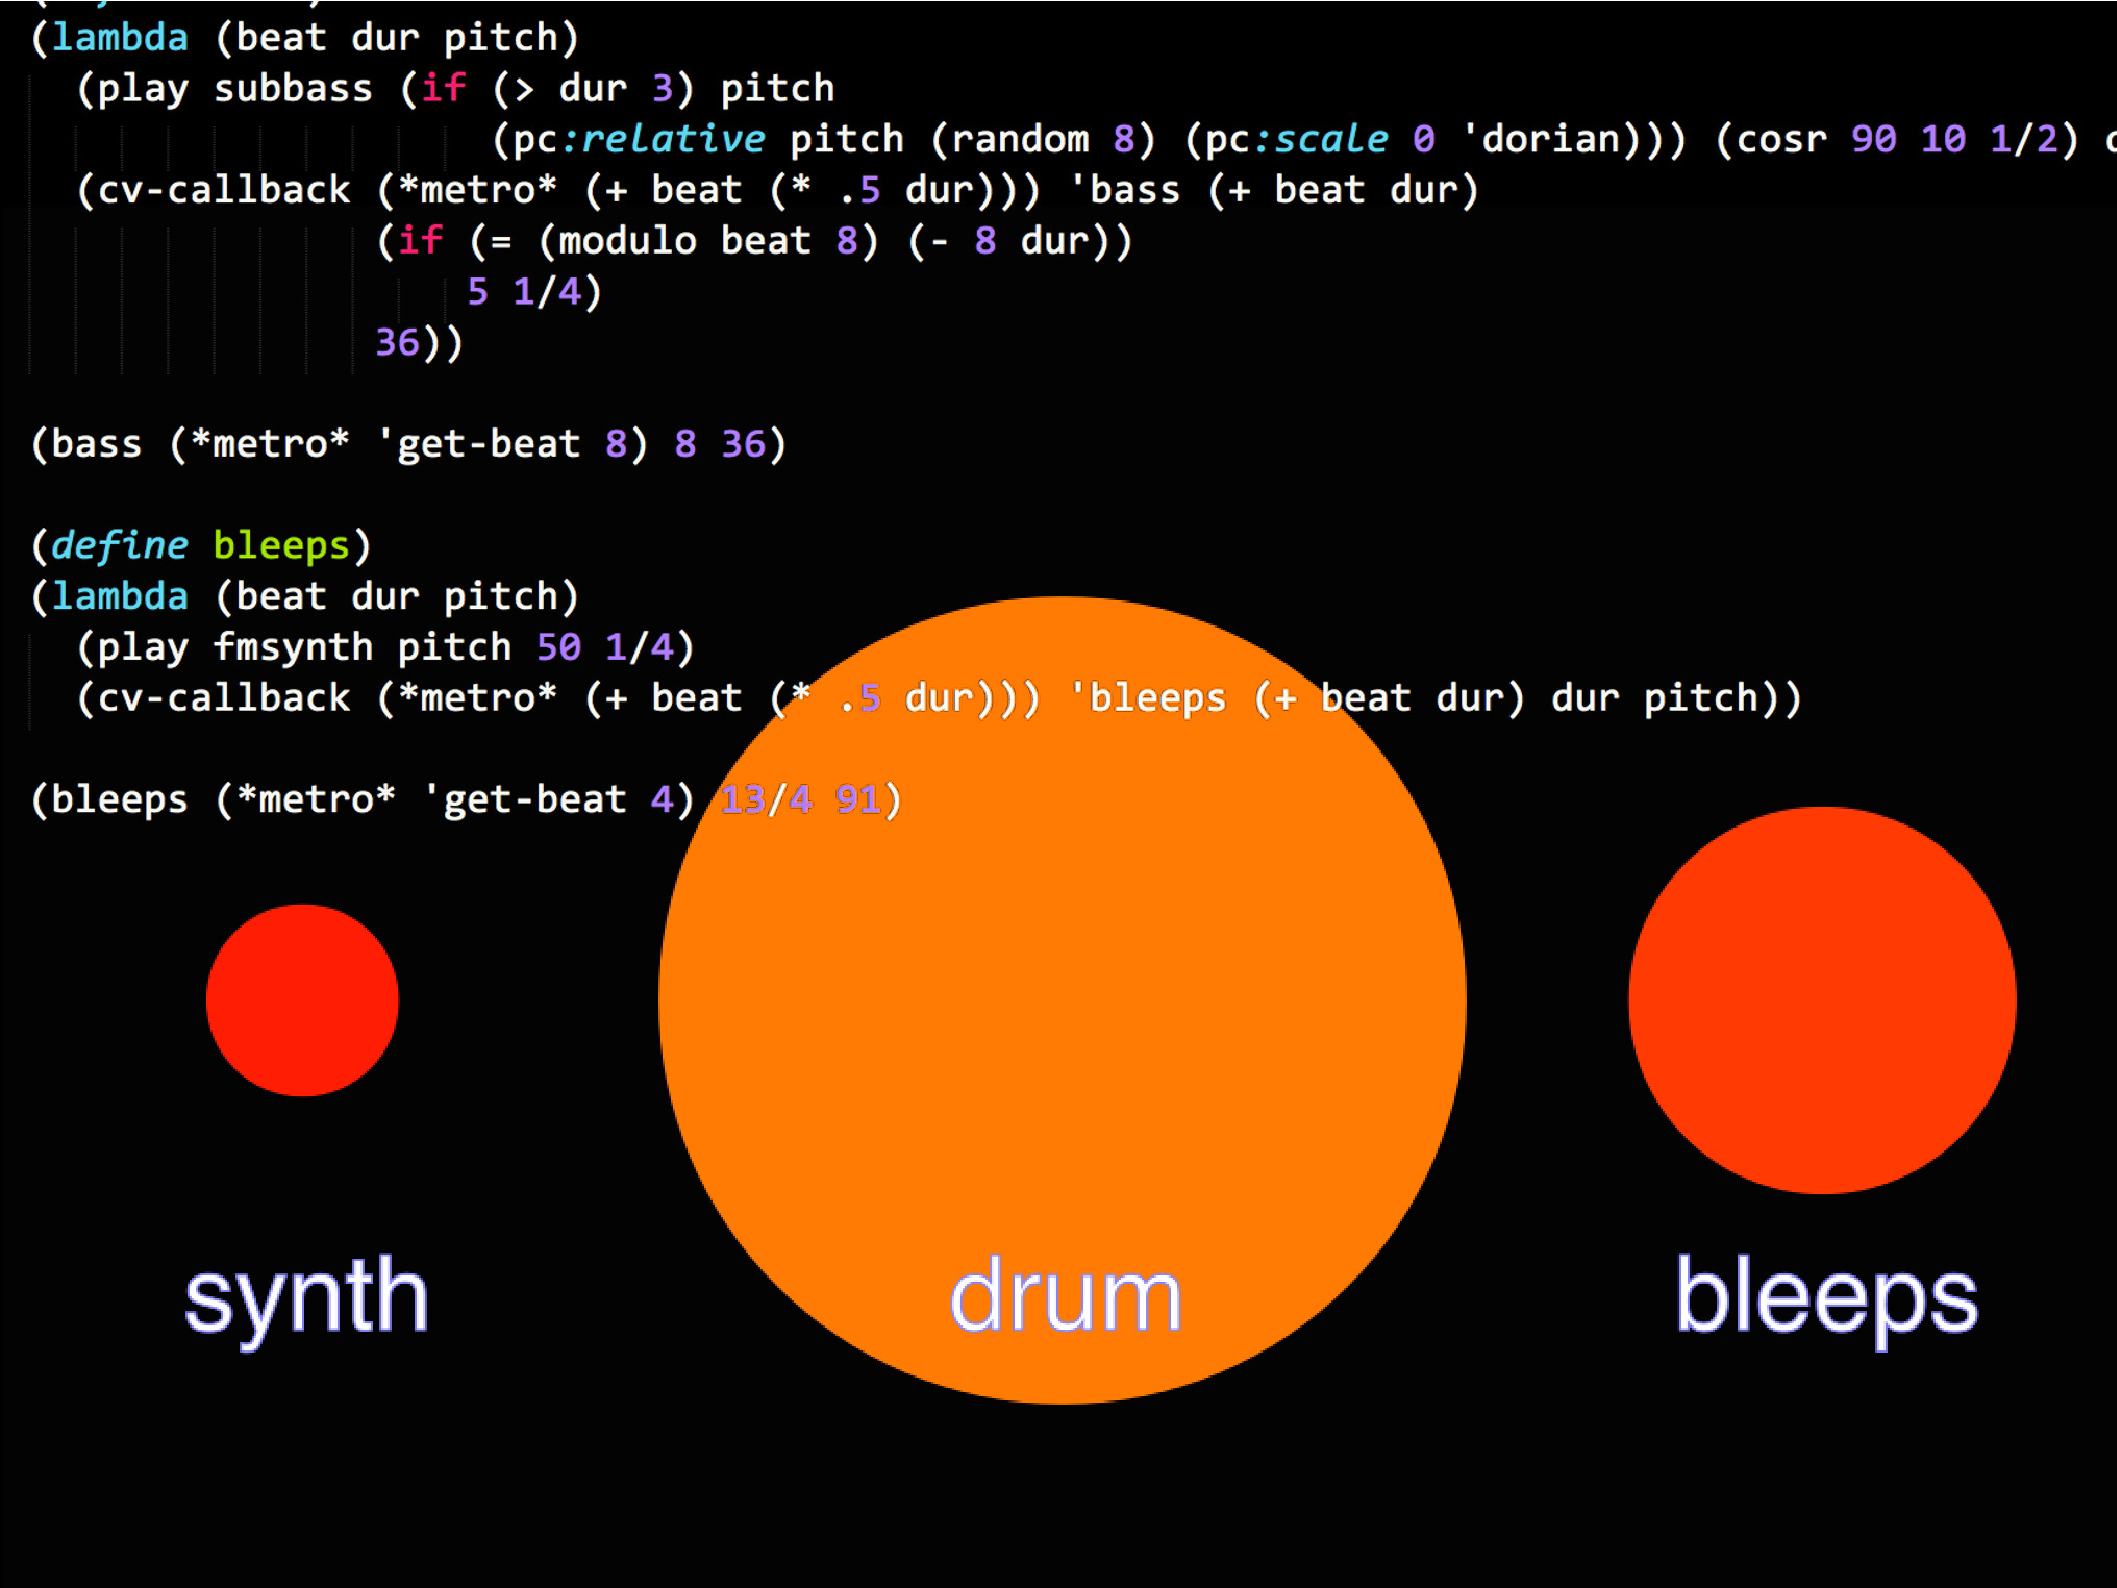
\includegraphics[width=.95\linewidth]{../study-2/results/visualisations/didactic-vis-overlay}
  \caption{Didactic visualisation}
  \label{fig:didactic-overlay}
\end{subfigure}%
\begin{subfigure}{.5\textwidth}
  \centering
  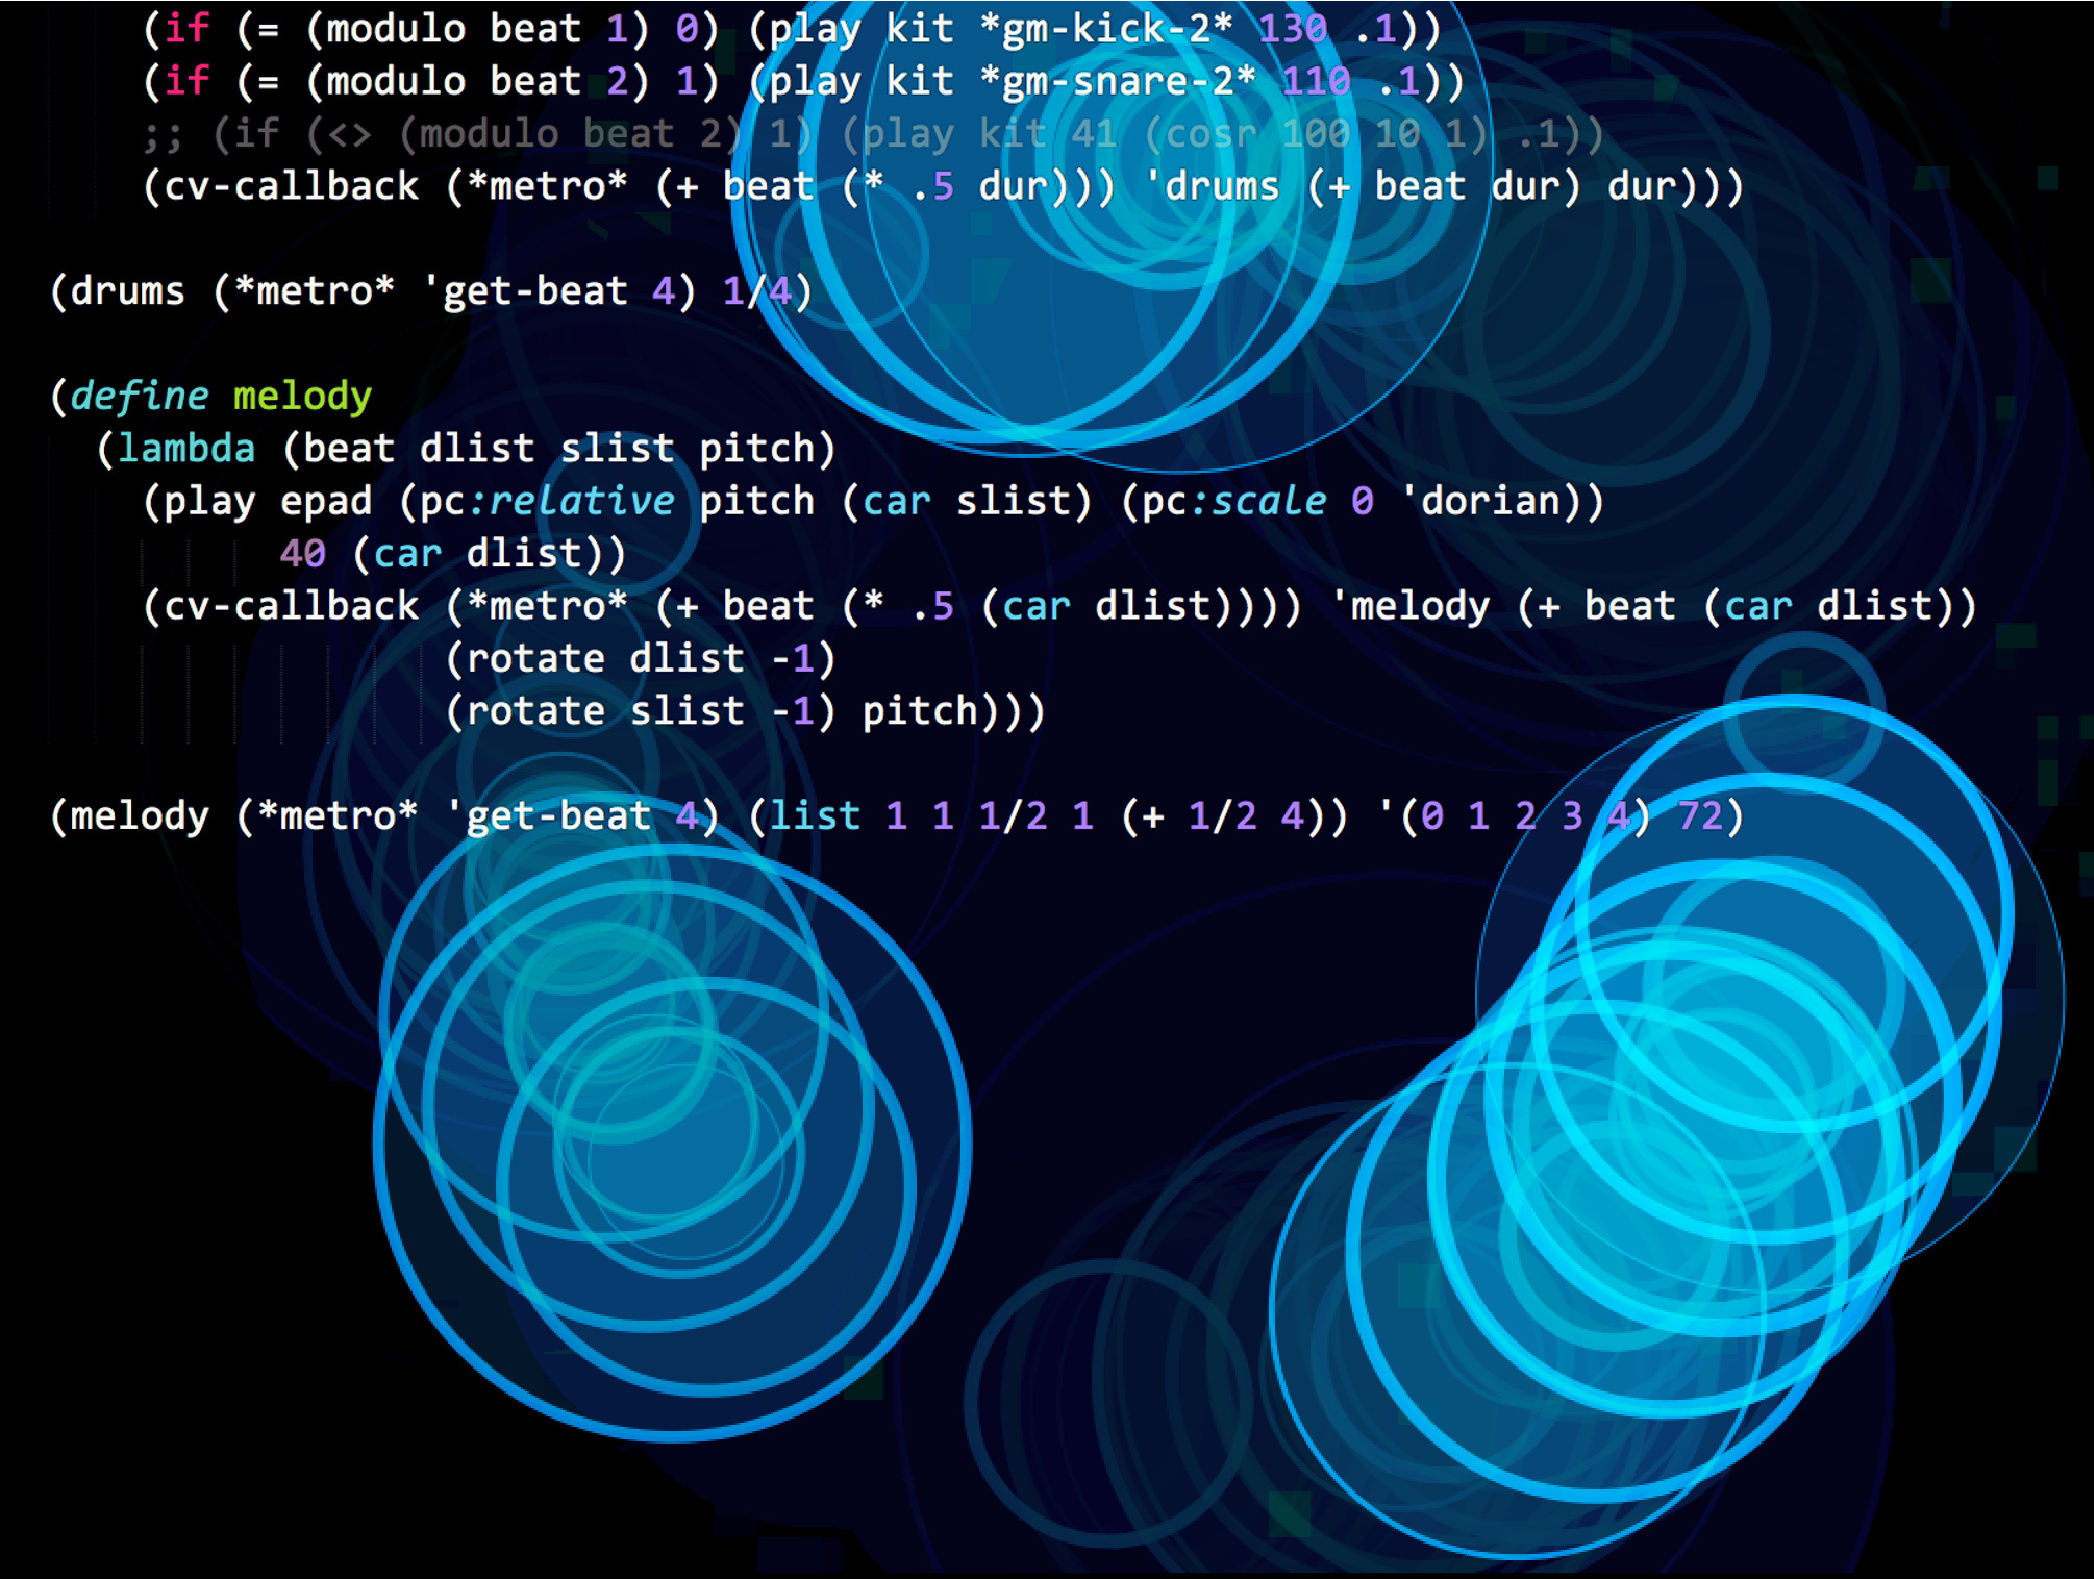
\includegraphics[width=.95\linewidth]{../study-2/results/visualisations/aesthetic-vis-overlay}
  \caption{Aesthetic visualisation}
  \label{fig:aesthetic-overlay}
\end{subfigure}

\caption[Visualisations with source code overlay]{Visualisations as they appeared during the study. Source code is overlayed on the visualisations.}
\label{fig:visualisation-overlay}
\end{figure}


\section{Method}

Two independent audiences ($N=19+22=41$) recruited through an on-campus advertisement (see Appendix~\ref{appendix:user-study-advertisement}) each watched a live coder perform two ten-minute ``sets'': one accompanied by the didactic visuals, and one with the aesthetic. The order of presentation of the two visual conditions was swapped between the groups. The improvisational nature of a live coding performance makes ``controlled'' experiments difficult, but the live coding artist attempted (as much as possible) to do the same two performances for each group.

Over the course of these performances, each audience member completed a survey (see Appendix~\ref{appendix:user-study-survey}) consisting of four sections: demographic information, their opinion of the first piece, their opinion of the second piece and questions about the performance overall. Similar to the first field trial, the survey primarily focussed on self-reported levels of ``enjoyment'' and ``understanding'' related to the visualisations specifically and also to the performance more generally. There was also a free-form question for suggested improvements to the visualisations.

After the laboratory study, to further inform the outcomes of the experiment, a video-cued recall~\cite{Suchman1992} interview was conducted using a video of the performance. Two of the performances were examined critically to assess the advantages and limitations of the visualisations.

\section{Participants}

Of the 41 participants who took part in the study over the two performances, 19 participants observed the first performance and 22 participants observed the second performance. The demographic makeup of the audiences was similar.

$66\%$ of the participants were male and most participants were aged between 18 and 32 ($76\%$). As the study was conducted within the Computer Science Department, a large proportion of the participants were experienced with programming with $90\%$ having current or previous experience with it. Nevertheless, only $15\%$ of participants had previous experience with any of the Lisp style of languages, the style used within the performance.

Of the participants, $68\%$ stated that they listened to a large amount of music though only about $15\%$ of participants stated that they played an instrument or sang regularly. $78\%$ of the participants had never seen a live coding performance before.

\begin{figure}
  \centering
  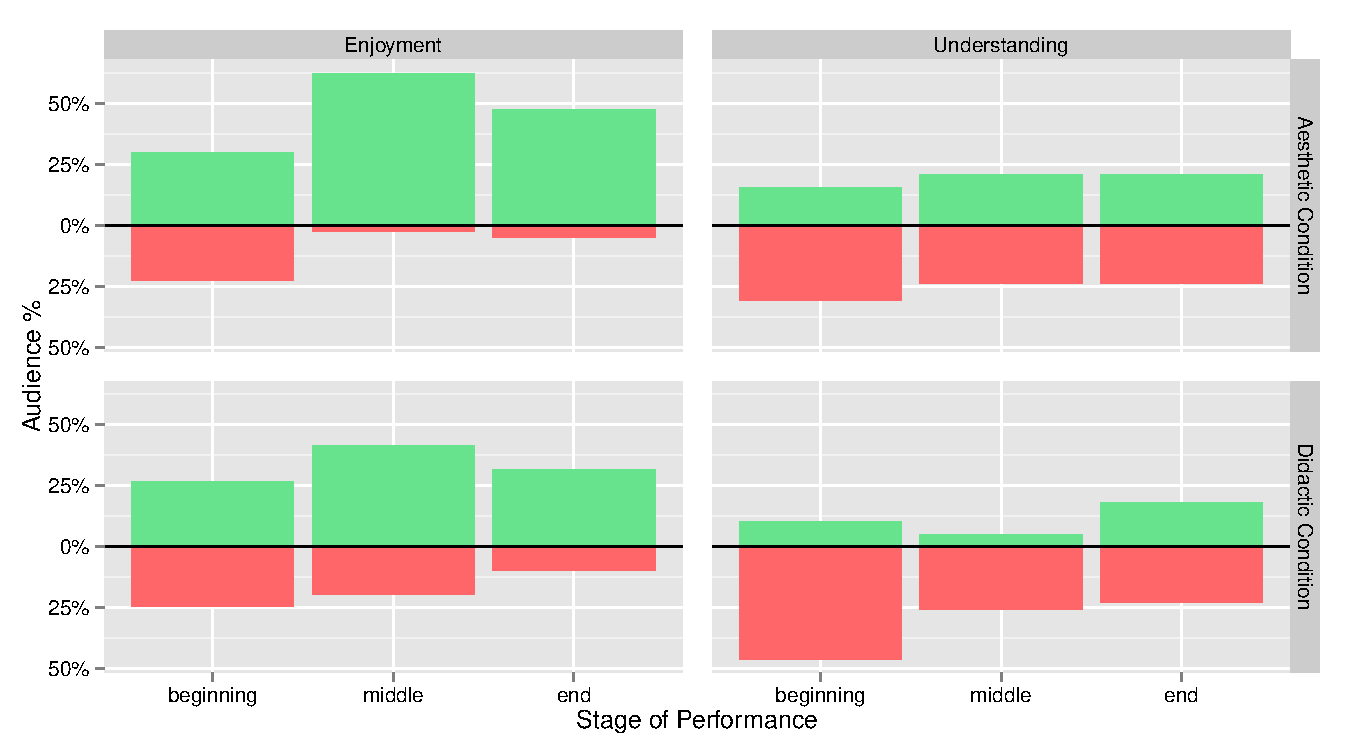
\includegraphics[width=\columnwidth]{../study-2/results/graphs/dimension-condition.pdf}
  \caption[User study survey condition and dimension results]{User study survey condition and dimension results. Percentage of the audience reporting ``high'' (green - above the line) and ``low'' (red - below the line) enjoyment and understanding over the beginning, middle and end stages of the performances for the aesthetic and didactic conditions. The remaining population, not shown here, reported ``medium'' levels of enjoyment or understanding.}
  \label{fig:dimension-condition}
\end{figure}

\section{Results}

The audience-reported enjoyment and understanding responses from the survey were evaluated for the two visualisation conditions as described below. A significance level of $0.05$ was used for the Chi-squared analysis.

\subsection{Enjoyment}

\begin{figure}
\centering
\begin{subfigure}{\textwidth}
  \centering
  \includegraphics[width=\columnwidth,page=4]{../images/graphs/condition-dimension.pdf}
  \caption[Didactic condition enjoyment detailed survey results]{Audience reported enjoyment level for the \textbf{didactic} condition.}
  \label{fig:didactic-enjoyment}
\end{subfigure}\\
\begin{subfigure}{\textwidth}
  \centering
  \includegraphics[width=\columnwidth,page=3]{../images/graphs/condition-dimension.pdf}
  \caption[Aesthetic condition enjoyment detailed survey results]{Audience-reported enjoyment level for the \textbf{aesthetic} condition.}
  \label{fig:aesthetic-enjoyment}
\end{subfigure}

\caption[User study enjoyment survey responses]{Audience reported enjoyment during the beginning, middle and end of the performance for the didactic and aesthetic visualisation conditions. Line width at each stage indicates proportion of the audience reporting high, medium or low enjoyment, and line colour connecting each section of the performance is determined by the enjoyment level at the \emph{beginning} of the performance.}
\label{fig:user-study-condition-enjoyment}
\end{figure}

Overall, the majority of the participants reported that both visualisation conditions had a positive effect on their \textbf{enjoyment} of the performance: $76\%$ stated that the aesthetic visualisations improved their enjoyment and $56\%$ stated that the didactic visualisations improved their enjoyment. No significant difference between the visualisation types regarding  enjoyment was found ($\chi^2=3.7733,df=2,p=0.1516$).

Participants were asked to rate their enjoyment during the (self-determined) ``beginning'', ``middle'' and ``end'' of the performances (see Figure~\ref{fig:user-study-condition-enjoyment}). The aesthetic visualisation resulted in a larger
percentage (around $60\%$) of the audience reporting high enjoyment during the middle of the performance compared to the didactic visualisation (around $40\%$). Notably, only a very small percentage reported low enjoyment for the aesthetic visualisations during the middle and end of the performance.

During the didactic performance, $15\%$ of the audience stated that their enjoyment \emph{increased} from the beginning of the performance and was steady thereafter. By contrast, $24\%$ of the audience reported this pattern of enjoyment during the aesthetic performance. Approximately $30\%$ of the audience of all (aesthetic and didactic) performances stated that their enjoyment remained steady throughout.

\subsection{Understanding}
\label{section:user-study-understanding}

\begin{figure}
\centering
\begin{subfigure}{\textwidth}
  \centering
  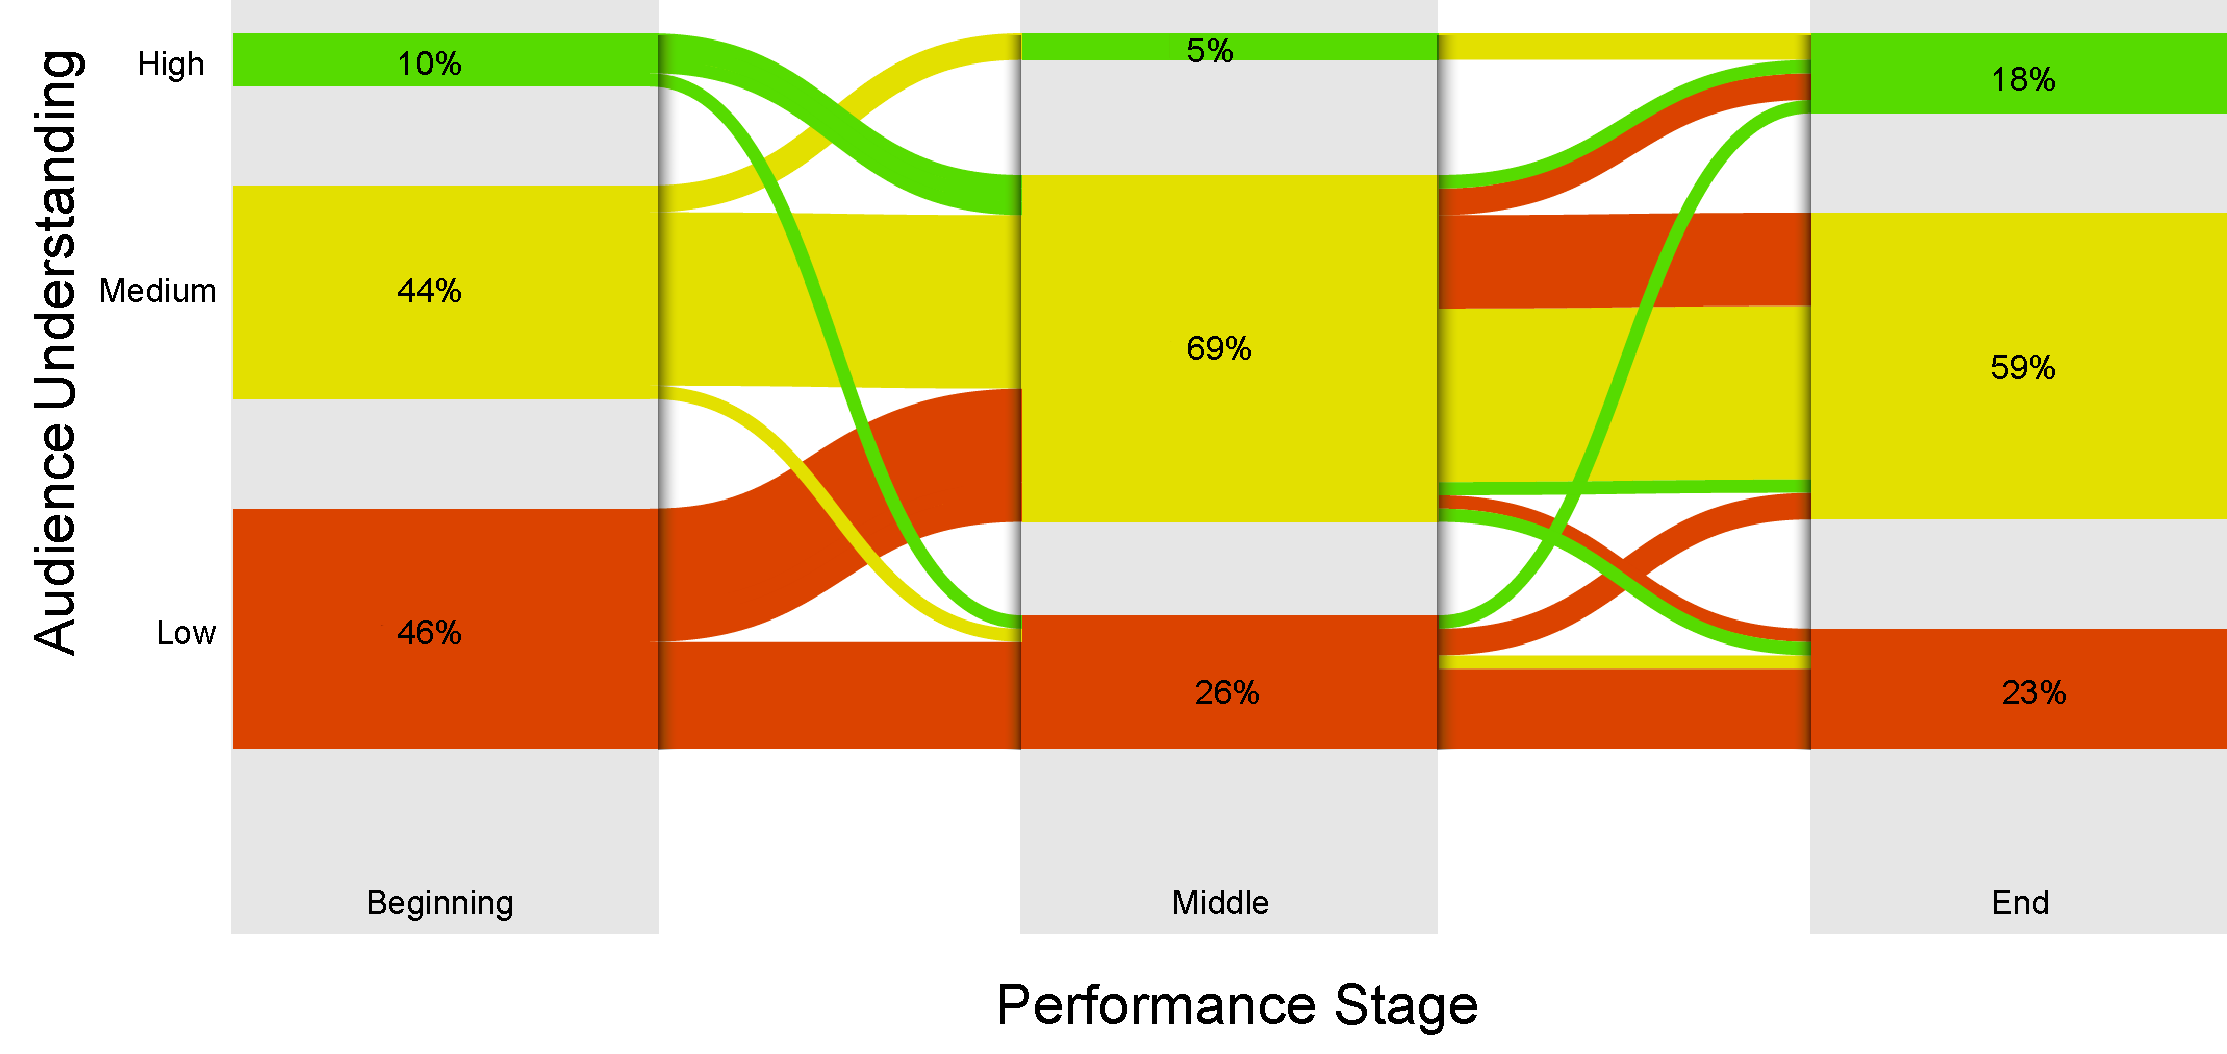
\includegraphics[width=\columnwidth,page=1]{../images/graphs/condition-dimension.pdf}
  \caption[Didactic condition understanding detailed survey results]{Audience reported understanding level for the \textbf{didactic} condition.}
  \label{fig:didactic-understanding}
\end{subfigure}\\
\begin{subfigure}{\textwidth}
  \centering
  \includegraphics[width=\columnwidth,page=2]{../images/graphs/condition-dimension.pdf}
  \caption[Aesthetic condition understanding detailed survey results]{Audience-reported understanding level for the \textbf{aesthetic} condition.}
  \label{fig:aesthetic-understanding}
\end{subfigure}

\caption[User study understanding survey responses]{Audience reported understanding during the beginning, middle and end of the performance for the didactic and aesthetic visualisation conditions. Line width at each stage indicates proportion of the audience reporting high, medium or low understanding, and line colour connecting each section of the performance is determined by the understanding level at the \emph{beginning} of the performance.}
\label{fig:user-study-condition-understanding}
\end{figure}

In response to a specific survey question, $37\%$ of participants stated that overall, the didactic visualisations ``helped them to \textbf{understand} the code'', compared to $12\%$ of participants for the aesthetic visualisations. This was a significant difference between the visualisation conditions ($\chi^2=7.1986,df=2,p=0.02734$).

Again, participants were asked to rate their understanding during the (self-reported) ``beginning'', ``middle'' and ``end'' of the performance (see Figure~\ref{fig:user-study-condition-understanding}). The aesthetic visualisation resulted in a smaller percentage of the audience (around $30\%$) reporting low understanding at the beginning of the performance compared to the didactic visualisations (around $45\%$). However, by the end of the performances both distributions looked very similar indeed.

During the didactic and aesthetic performances, $49\%$ and $44\%$ respectively of the participants stated that their understanding \emph{remained the same} throughout the performances. During the didactic performance, $10\%$ of the audience reported a level of understanding that \emph{trended downwards} (eg. high to low) compared to $20\%$ of the audience during the aesthetic performance. However, this reported advantage of the didactic visualisations was offset by the reported audience understanding at the beginning of the performance where $44\%$ indicated a low understanding with the didactic visualisations compared to only $30\%$ with the aesthetic visualisations. 

Overall, the survey results for audience understanding are complex, and reported levels of understanding fluctuated during the performances. Dramatically, Figure~\ref{fig:didactic-understanding} shows that a very small proportion of the audience reported high understanding during the middle of the performances. One interpretation of this result might be that it took audience members some time to work out what the didactic visualisations were actually showing, and that this conflicted with the first impressions of what some audience members assumed (hence the decrease in levels of understanding from beginning to middle). However, once they finally understood the graphics some audience members were then able to better understand the live-coding performance.

\subsection{Liveness}
\label{section:liveness}

Participants were asked to discuss how each visualisation influenced or impacted the liveness of the performance. Concepts identified included positive and negative valence towards the didactic visualisations, positive and negative valence towards the aesthetic visualisations and the relevance of visual source code. The discussion included the positive and negative aspects of the didactic visualisations, the positive and negative aspects of the aesthetic visualisations, source code discussion, and statements indicating an understanding between the visuals and the source code.

Overall, $54\%$ of the audience indicated negative valence towards the didactic visualisation regarding liveness, citing a variety of reasons including that the ``visuals only responded to what was typed'', that the ``musical forms didn't occur at the most expected times'' and that the visualisations ``perhaps made the performance seem too polished''.

On the other hand, $34\%$ of the audience indicated positive valence towards the didactic visualisations suggesting that ``it was easier to follow this visualisation than the code'', ``the visualisations clearly showed the changes being made to the code'' and that these visualisations ``helped more with communicating that the performance was live''.

$40\%$ of the audience had negative valence towards the aesthetic visualisation's effect on the sense of liveness. Reasons cited include that the ``influence is not clear'' between the code and the visuals, that ``the visualisation did not make much sense'' and that the ``visualisations did nothing to suggest that the performance was live''.

$32\%$ had positive valence towards the aesthetic visualisation. Responses included that these visuals were ``less dominating and more complementary'' and that ``the visualisations helped to show when a piece of code started working''.

A relatively large proportion ($28\%$) of the audience discussed the importance of the source code to the sense of liveness of the performance such as that the ``code showed what the musician was doing physically''. A further $5\%$ of the audience demonstrated a deeper understanding of the live coding process such as ``changing values produced changes in tone and speed of the music pitch''.

\subsection{Improvements}
\label{section:improvements}

The audience was asked to indicate possible improvements to the visualisations. 40\% of the audience suggested improvements that indicated a desire to see a better relationship between the visualisations and the music, with suggestions such as matching the visualisations to musical rhythms or pitch. For example, one audience member stated that the visualisations should ``perhaps have a stronger correlation with hush tones and defined shapes, baselines with wide and soft shapes with animations that follow the beat more consistently''.

Other members of the audience stated that they would like to see a better relationship between the code and the visuals. For example, one audience member stated that ``it would be really cool once you edit a code line and then activate it for it to morph into a visualisation for as long as this line of code is active''. Another audience member stated that ``it would be better to not just relate the function to the sound but relate every beat to the sound or to the code responsible for that beat''.

Other suggestions included increasing the readability of source code, increased immediacy of actions, increasing uniformity between the visualisations, and the use of images to assist with the understanding of high level concepts.

\subsection{Follow-Up Interview}
\label{section:study-2-follow-up-interview}

A follow-up interview was conducted with the live coder to further examine the visualisation approach taken and the overall usability of the visualisations. See Appendix~\ref{appendix:live-coder-interview-transcript} for the full interview transcript.

\section{Discussion}
\label{section:user-study-discussion}

The overall enjoyment of the visualisations was high, for both the aesthetic and didactic visualisations. Reported enjoyment of the aesthetic visualisations was higher than for the didactic visualisations but the trends across Figures~\ref{fig:aesthetic-understanding} and~\ref{fig:didactic-understanding} for understanding are complex.

As discussed above, the small number of high responses for understanding during the middle of the didactic performances, and the decreasing trend from high to middle level understanding from beginning to middle of the performances perhaps indicates a higher cognitive load for understanding the didactic visualisations themselves. In fact, features of the didactic visualisation were reported to confuse some members of the audience, despite their stated aim of \emph{assisting} audience understanding. One audience member even stated that they ``found them distracting'' and that they ``preferred just to read the code''.
 
The video-cued-recall interview indicated that the live coder's experience of the visualisations was fundamentally different to that of the audience. While many members of the audience reported that they drifted between focussing on the music, focussing on the visualisations and focussing on the code, the live coder reported that his focus was purely on the code and the music, rarely drifting. In one particular section of the interview, the live coder stated: ``I definitely wasn't paying attention to them [the visualisations] on the day. In fact I tune them out as best I can because I am just trying to focus on the code''. By contrast, one audience member stated that ``you could see the code being written and the visualisations helped to show when a piece of code started working''. Another audience member stated that ``the visualisations were interesting but distracting''. When asked if the visualisations were distracting, the live coder stated: ``Ah, no. In general I'm just so focussed on the code''.


\subsection{Limitations}

Several limitations of the investigation method were identified. 

It should be noted that there are inherent difficulties in evaluating a live performance. Notably, physical factors such as constraints on the number of projectors, time during which to perform and live coder fatigue could have impacted the results. Similarly, factors such as musical preference, musical style and variations in the musical performance could have contributed to audience reception of the performance. 

Due to the time and fatigue constraints of the live performance, no baseline for the study was set. Evaluation of the visualisations in comparison to a non-visualised live performance would be required to determine if the visualised live performance provided an additional benefit to understanding or enjoyment. In this case however, the comparison of the two live coding techniques provided a useful and valid basis on which to develop a second visualisation prototype for further evaluation.

The impact of testing effects on the validity of the study due to the order the two conditions were presented to the audience were mitigated through order balancing. However, differences between the live coding performances are inherent. The live coder attempted, to the best of his ability, to keep the performances consistent.

\section{Summary}

The differences between the experience of the live coder and the experience of the audience were identified during the follow-up interview with the live coder. The live coder had a mental image of the active code and the structure of the program that was not being communicated through the source code. Visualisations assisted the audience in some regards as to the state of the program, however, it was hypothesised that more effective visualisation techniques might take advantage of the mental model of the live coder and attempt to align the audience with this mental model.

Results of this study indicate that there is a need for further refinement and evaluation of visualisations with specific focus on elucidating the state of the active program through the alignment of mental models between the live coder and the audience.

% -list the results of this study

% -link to the next iteration of the visualisations - what were the most important limitations with the evaluation process that had to be identified and what were the most important limitations with the visualisations that were identified to be addressed in the next study.



